\documentclass[tikz,border=10pt]{standalone}
\usepackage{tikz}
\usetikzlibrary{arrows.meta}

\tikzset{
  sfgsource/.style={circle, draw=green!60!black, line width=1.2pt, minimum size=0.95cm, inner sep=0pt},
  sfgnode/.style={circle, draw=purple!70!black, line width=1.2pt, minimum size=0.95cm, inner sep=0pt},
  sfgsink/.style={circle, draw=red!70!black, line width=1.2pt, minimum size=0.95cm, inner sep=0pt},
  sfgedge/.style={->, line width=1.2pt, draw=black!80, >=Stealth},
  gain/.style={font=\small\itshape, fill=white, inner sep=1pt}
}

\begin{document}
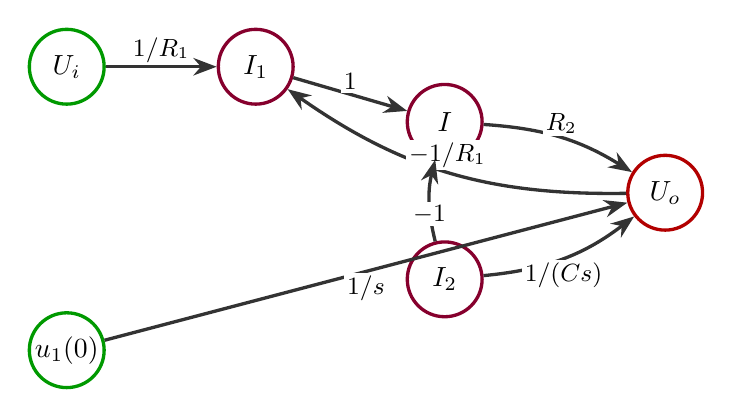
\begin{tikzpicture}
  \node[sfgsource] (ui) at (0,1.8) {$U_i$};
  \node[sfgsource] (u0) at (0,-1.8) {$u_1(0)$};
  \node[sfgnode] (i1) at (2.4,1.8) {$I_1$};
  \node[sfgnode] (i) at (4.8,1.1) {$I$};
  \node[sfgnode] (i2) at (4.8,-0.9) {$I_2$};
  \node[sfgsink] (uo) at (7.6,0.2) {$U_o$};

  \draw[sfgedge] (ui) -- node[gain, above] {$1/R_1$} (i1);
  \draw[sfgedge, bend left=18] (uo) to node[gain, above] {$-1/R_1$} (i1);
  \draw[sfgedge] (i1) -- node[gain, above] {$1$} (i);
  \draw[sfgedge, bend left=14] (i2) to node[gain, below] {$-1$} (i);
  \draw[sfgedge, bend left=14] (i) to node[gain, above] {$R_2$} (uo);
  \draw[sfgedge, bend right=16] (i2) to node[gain, below] {$1/(Cs)$} (uo);
  \draw[sfgedge] (u0) -- node[gain, below] {$1/s$} (uo);
\end{tikzpicture}
\end{document}
